
% This LaTeX was auto-generated from an M-file by MATLAB.
% To make changes, update the M-file and republish this document.

\documentclass{article}
\usepackage{graphicx}
\usepackage{color}

\sloppy
\definecolor{lightgray}{gray}{0.5}
\setlength{\parindent}{10pt}
\usepackage[margin=1in]{geometry}

\begin{document}

\title{spikesort for Kontroller}
\author{Srinivas Gorur-Shandilya}
\maketitle

    
    
\subsection*{Contents}

\begin{itemize}
\setlength{\itemsep}{-1ex}
   \item Tests and Performance Metrics
   \item Test Data 1
   \item Comparison of PCA and t-SNE
   \item Quantification of Errors: A spike
   \item Quantification of Errors: B spike
   \item Version Info
\end{itemize}


\subsection*{Tests and Performance Metrics}

\begin{par}
In this document, we test how good spikesort is, and measure the error rate on some carefully annotated data.
\end{par} \vspace{1em}


\subsection*{Test Data 1}

\begin{par}
In this data, A and B neurons have very similar amplitudes, and the recording was performed in LFP mode (no low pass filter). Thus, spikes were detected in the positive peaks. This is what the actual data looks like:
\end{par} \vspace{1em}

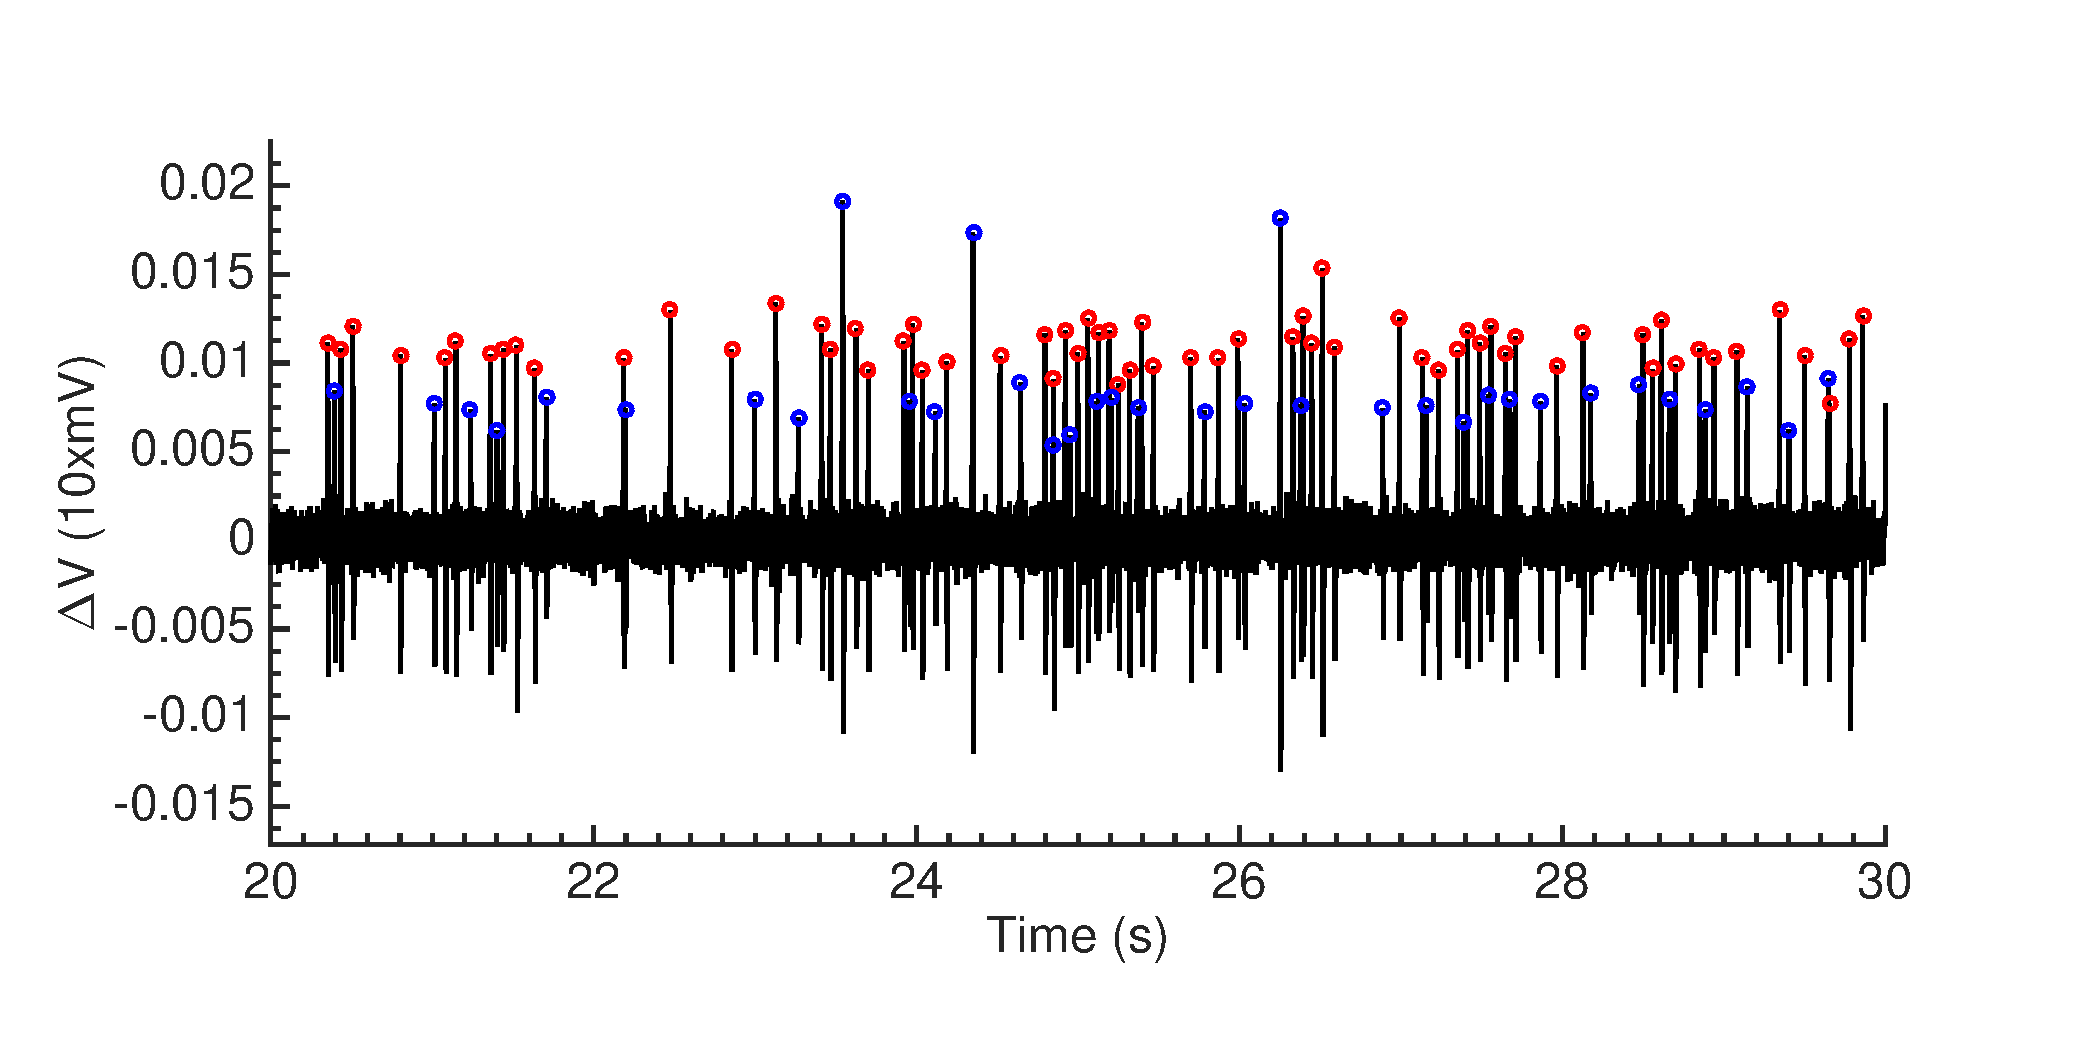
\includegraphics [width=\textwidth]{makeTestReport_01.pdf}
\begin{par}
The large B spikes are coincident A and B spikes, and are counted as such.
\end{par} \vspace{1em}


\subsection*{Comparison of PCA and t-SNE}

\begin{par}
In the following figure, we plot rasters of the manually inspected data, and compare it to the best PCA solution and the best t-SNE solution:
\end{par} \vspace{1em}

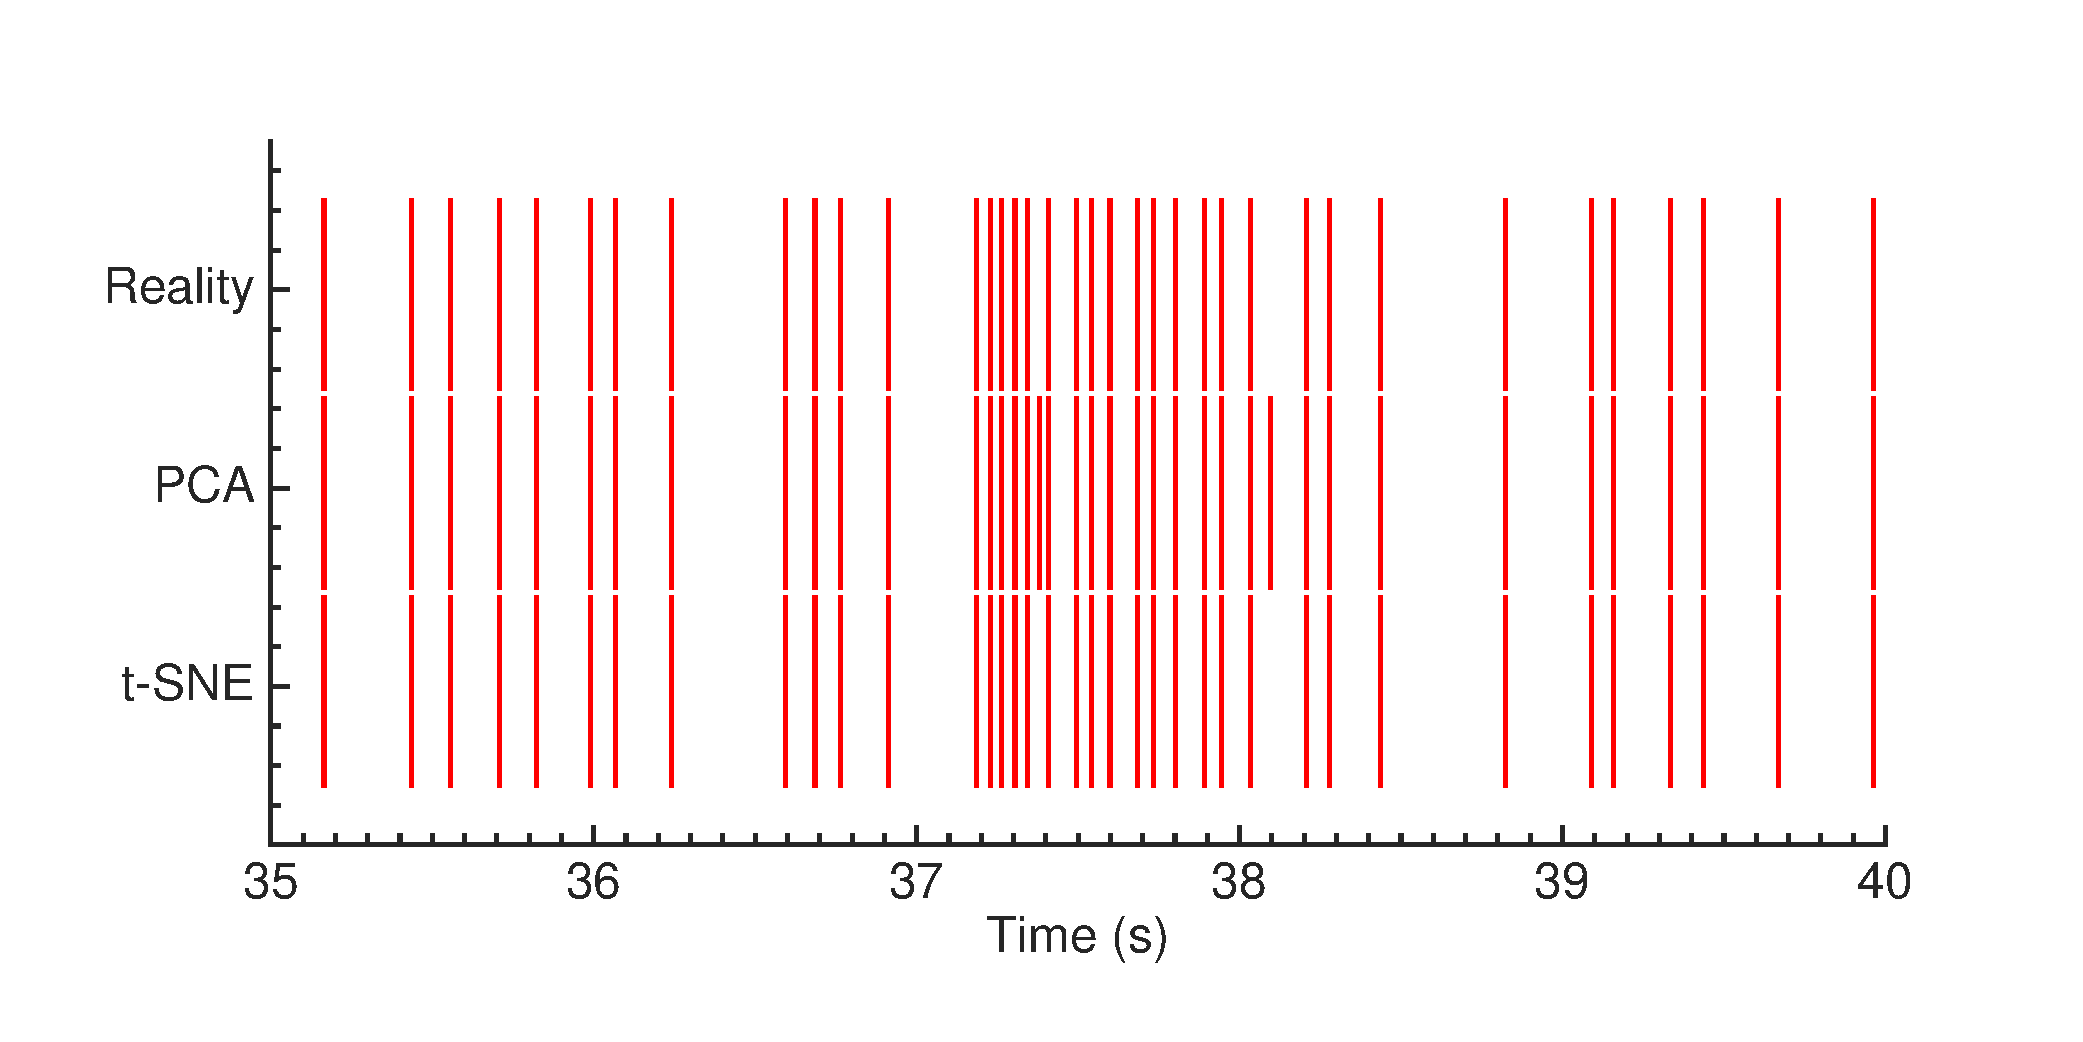
\includegraphics [width=\textwidth]{makeTestReport_02.pdf}
\begin{par}
In this view, the best PCA solution has a few extra A spikes that should not be there.
\end{par} \vspace{1em}
\begin{par}
In the next figure, we compare how PCA and t-SNE achieve dimensionality reduction on the same data. As can be seen, the clusters overlap significantly in PCA, while the clusters are well separated in t-SNE. The three main clusters correspond to noise, the B-neuron and the A-neuron. Smaller clusters correspond to simultaneous or otherwise co-mingled spikes.
\end{par} \vspace{1em}
\begin{par}

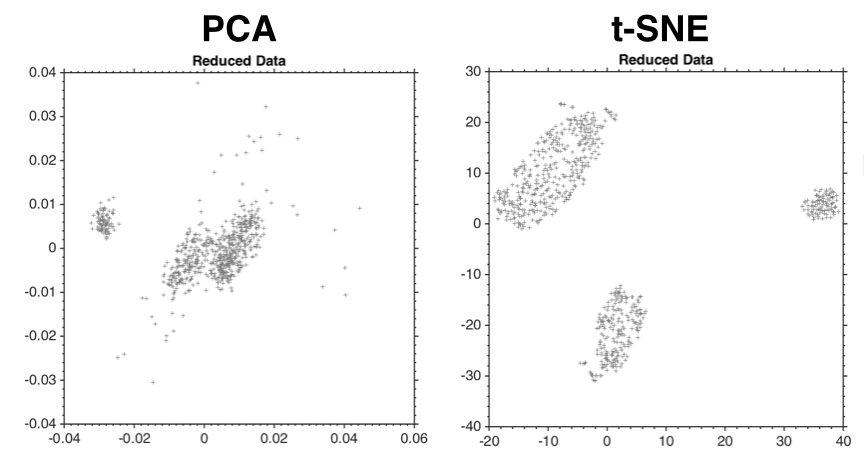
\includegraphics [width=\textwidth]{dim-red.png}

\end{par} \vspace{1em}


\subsection*{Quantification of Errors: A spike}

\begin{par}
We now quantify the errors made by each method on this dataset.
\end{par} \vspace{1em}
\begin{par}
The fraction of A spikes correctly identified by the PCA algorithm is:
\end{par} \vspace{1em}

        \color{lightgray} \begin{verbatim}99.3
\end{verbatim} \color{black}
    \begin{par}
The fraction of A spikes correctly identified by the t-SNE algorithm is:
\end{par} \vspace{1em}

        \color{lightgray} \begin{verbatim}99.5
\end{verbatim} \color{black}
    \begin{par}
The fraction of A spikes reported by PCA that actually match to a A spikes is:
\end{par} \vspace{1em}

        \color{lightgray} \begin{verbatim}98.3
\end{verbatim} \color{black}
    \begin{par}
The fraction of A spikes reported by t-SNE that actually match to a A spikes is:
\end{par} \vspace{1em}

        \color{lightgray} \begin{verbatim}100
\end{verbatim} \color{black}
    

\subsection*{Quantification of Errors: B spike}

\begin{par}
We now quantify the errors made by each method on this dataset.
\end{par} \vspace{1em}
\begin{par}
The fraction of B spikes correctly identified by the PCA algorithm is:
\end{par} \vspace{1em}

        \color{lightgray} \begin{verbatim}95.8
\end{verbatim} \color{black}
    \begin{par}
The fraction of A spikes correctly identified by the t-SNE algorithm is:
\end{par} \vspace{1em}

        \color{lightgray} \begin{verbatim}100
\end{verbatim} \color{black}
    \begin{par}
The fraction of B spikes reported by PCA that actually match to a B spikes is:
\end{par} \vspace{1em}

        \color{lightgray} \begin{verbatim}94.4
\end{verbatim} \color{black}
    \begin{par}
The fraction of B spikes reported by t-SNE that actually match to a B spikes is:
\end{par} \vspace{1em}

        \color{lightgray} \begin{verbatim}99.5
\end{verbatim} \color{black}
    

\subsection*{Version Info}

\begin{par}
The file that generated this document is called:
\end{par} \vspace{1em}

        \color{lightgray} \begin{verbatim}makeTestReport
\end{verbatim} \color{black}
    \begin{par}
and its md5 hash is:
\end{par} \vspace{1em}

        \color{lightgray} \begin{verbatim}9357a9e083951fb117f9ce4b1e9ff248
\end{verbatim} \color{black}
    \begin{par}
This file should be in this commit:
\end{par} \vspace{1em}

        \color{lightgray} \begin{verbatim}6079dbdec41762d6b2198a4c6361dc05ac65ba2b

\end{verbatim} \color{black}
    \begin{par}
This document was built in:
\end{par} \vspace{1em}

        \color{lightgray} \begin{verbatim}7.12 seconds.
\end{verbatim} \color{black}
    


\end{document}
    
